\documentclass{standalone}
\usepackage{tikz}
\usepackage{ctex,siunitx}
\usepackage{tkz-euclide}
\usepackage{amsmath}
\usetikzlibrary{patterns, calc}
\usetikzlibrary {decorations.pathmorphing, decorations.pathreplacing, decorations.shapes,}
\begin{document}
\small
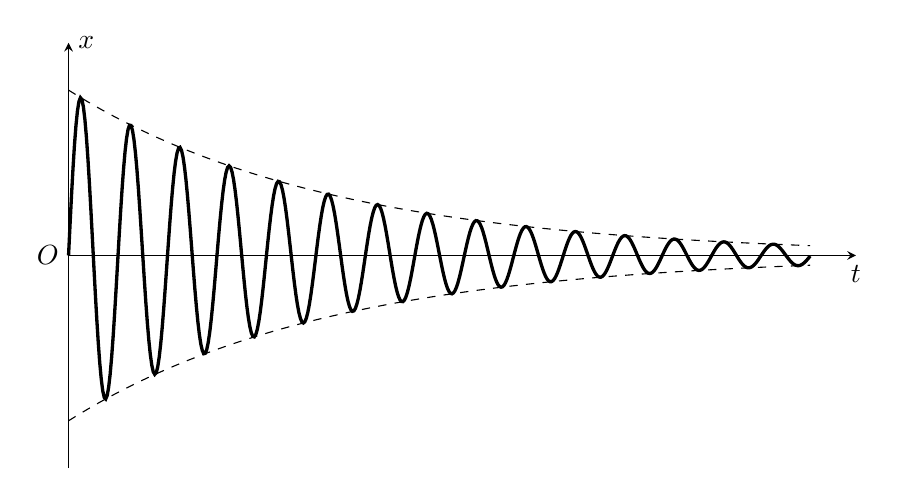
\begin{tikzpicture}[>=stealth, yscale=3, domain=0:3*pi, samples=500]
  \draw [->](0,0)node [left]{$O$}--(10,0) node [below]{$t$};
  \draw [->](0,-0.9)--(0,0.9) node [right]{$x$};
  \draw [very thick]  plot (\x,{exp(-.3*\x)*sin(10*\x r)*0.7});
  \draw [dashed]  plot (\x,{exp(-.3*\x)*0.7});
  \draw [dashed]  plot (\x,{-exp(-.3*\x)*0.7});
\end{tikzpicture}
\end{document}